\chapter{zzz Template for ElmerGUI Tutorials}

\modinfo{Directory}{Template}
\modinfo{Solvers}{\Idx{HeatSolve}, \Idx{FlowSolve}}
\modinfo{Tools}{\Idx{ElmerGUI}}
\modinfo{Dimensions}{zzz 2D,zzz Transient}
\modinfo{Author}{zzz Rich Bayless}


\subsection*{Introduction}

zzz This Template For Tutorials is designed to help make it easy to create a new tutorial using ElmerGUI.  Having an outline of a tutorial should allow for simpler development of new tutorials, and will help keep the look and feel of new tutorials in unison with existing tutorials.

zzz Anywhere you see `zzz', it means that section needs to be replaced.  Any text that begins with `zzz', should be deleted and replaced by the appropriate text for your tutorial.  

zzz Think of `zzz' as a spot where you should `fill in the blanks'.



\subsection*{Case definition}


zzz Enter your case definition here.

The geometry for this tutorial looks like as shown in figure \ref{fg:geometry}.

zzz Enter your geometry figure here.

\begin{figure}[H]
\centering
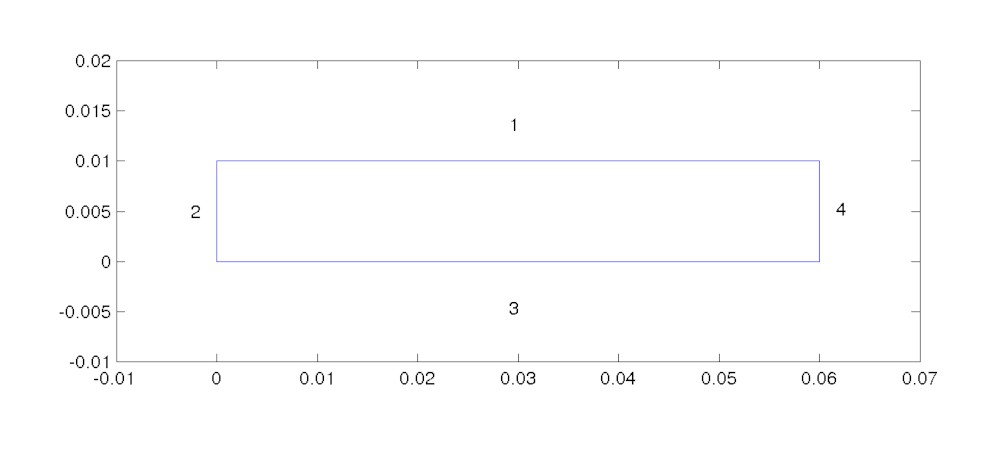
\includegraphics[width=0.8\textwidth]{geometry.png}
\caption{Geometry}\label{fg:geometry}
\end{figure}  

\subsection*{ElmerGUI Equation Menu}

zzz Note that we include both edf and edf-extra examples.  If you don't need the edf-extra example, the first section can be deleted.  It is suggested to keep the edf example, to show where the edf file comes from.

zzz The GUI definitions of zzz solver utilized in this tutorial are located in the \texttt{edf-extra} folder and thus need to be manually activated in the ElmerGUI.\\

zzz Note that the extra definition needs to be loaded first, before any other steps in building any tutorial.  Once the extra definition has been loaded, and the ElmerGUI project has been saved, then the reference to the extra definition will be stored in the project, and you won't have to load the extra definition again.

\begin{verbatim}
File
  Definitions
    Append -> zzz.xml
  Close
\end{verbatim}

\noindent The \texttt{\Idx{zzz.xml}} definition file is, by default, located in Linux in:

\texttt{\$ELMER\_HOME/share/ElmerGUI/edf-extra}

\noindent and in Windows, located in:

\texttt{C:/Program Files/Elmer 9.0-Release/share/ElmerGUI/edf-extra}\\

We will also be using the \Idx{zzz Solver}, which is one of the default, pre-loaded GUI definitions, so it does not need to be manually activated.  For reference, the  \texttt{\Idx{zzz.xml}} definition file is, by default, located in Linux in:

\texttt{\$ELMER\_HOME/share/ElmerGUI/edf}

\noindent and in Windows, located in:

\texttt{C:/Program Files/Elmer 9.0-Release/share/ElmerGUI/edf}\\


\subsection*{Solution procedure}

The mesh is given in ElmerGrid format in file \texttt{zzz}, load this file.

\ttbegin
File 
  Open -> zzz
\ttend

You should obtain your mesh and may check \texttt{Model Summary...} that it consists of zzz elements.  Your mesh should look like as shown in figure \ref{fg:mesh}

\begin{figure}[H]
\centering
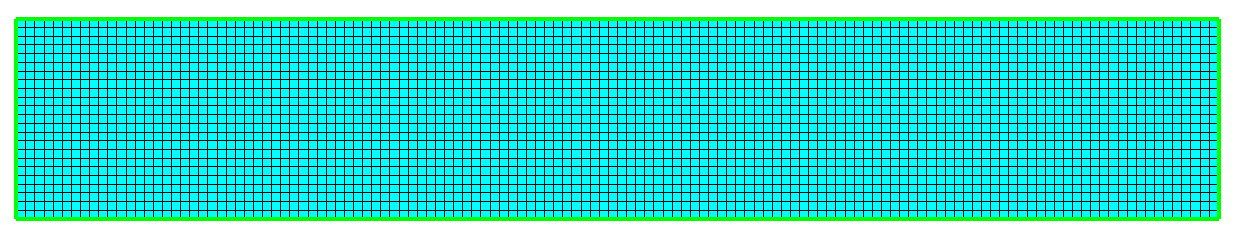
\includegraphics[width=0.8\textwidth]{mesh}
\caption{Mesh}\label{fg:mesh}
\end{figure}

After we have the mesh we start to go through the Model menu from the top to bottom.  In the Setup we choose things related to the whole simulation such as file names, time stepping, constants etc.  

The simulation is carried out in 2-dimensional Cartesian coordinates.

zzz 2nd order bdf time stepping method is selected with zzz steps and with step size of zzz seconds.

zzz Every menu selection section must be revised for each tutorial.  These examples show the proper format and typical content.

\ttbegin
Model
  Setup 
    Simulation Type = Transient
    Steady state max. iter = 20
    Time Step Intervals = 200
    Gravity = 0 -1 0 9.82
  Apply
\ttend

In the equation section we choose the relevant equations and parameters related to their solution. 

zzz In this case we'll have one set of equations (named ``Natural Convection'') which consists of the heat equation and of the Navier-Stokes equation.

When defining Equations and Materials it is possible to assign to the bodies immediately, or to use mouse selection to assign them later. In this case we have just one body and therefore its easier to assign the Equation and Material to it directly.  It is important to select the convection to be computed since that couples the velocity field to the heat equation.

zzz The system may include non-linear iterations of each equation and steady state iterations to obtain convergence of the coupled system. It is often a good idea to keep the number of non-linear iterations in a coupled case low. Here we select just one non-linear iteration for both equations.\\

For the linear system solvers we are happy to use the defaults. One may however, try out different preconditioners (ILU1,\ldots) or direct Umfpack solver, for example.

zzz Every menu selection section must be revised for each tutorial.  These examples show the proper format and typical content.
\ttbegin
Model
  Equation
   Name = Natural Convection
    Apply to Bodies = 1
    Heat Equation
      Active = on
    Add 
    OK
\ttend        
The Material section includes all the material parameters. They are divided into generic parameters which are direct properties of the material without making any assumptions on the physical model, such as the mass. Other properties assume a physical law, such as conductivities and viscosity. 

zzz Discuss which materials are used, why they are used, and any interesting details.
   
zzz Every menu selection section must be revised for each tutorial.  These examples show the proper format and typical content.

\ttbegin
Model
  Material
    Apply to Bodies = 1 
    Material library    
      Water (room temperature)
    General 
      Reference Temperature = 293
    Add
    OK
\ttend

A Body Force represents the right-hand-side of a equation. It is generally not a required field for a body. 

zzz In this case, however, we apply the buoyancy resulting from heat expansion as a body force to the Navier-Stokes equation.

zzz Every menu selection section must be revised for each tutorial.  These examples show the proper format and typical content.

\ttbegin
Model
  Body Force
    Name = Buoyancy
    Apply to Bodies = 1
    Navier-Stokes
      Boussinesq = on
    Add 
    OK
\ttend    

Initial conditions should be given to transient cases, and probably are not needed for steady state solutions. 

zzz In this case we choose a constant Temperature field and an small initial velocity that initializes the symmetry break. 

zzz Every menu selection section must be revised for each tutorial.  These examples show the proper format and typical content.

\ttbegin
Model
  Initial Condition 
    Name = Initial Guess
    Heat Equation
      Temperature = 293
    Navier-Stokes
      Velocity 1 = 1.0e-9
      Velocity 2 = 0.0
\ttend

Only one boundary condition may be applied to each boundary and therefore all the different physical BCs for a boundary should be grouped together. 

zzz In this case the Temperature and Velocity. The side walls are assumed to be adiabatic.

zzz Every menu selection section must be revised for each tutorial.  These examples show the proper format and typical content.

\ttbegin
Model
  BoundaryCondition
    Name = Bottom
    Heat Equation
      Temperature = 293.5
    Navier-Stokes 
      Velocity 1 = 0.0
      Velocity 2 = 0.0
    Add
    New

    Name = Top
    Heat Equation
      Temperature = 293
    Navier-Stokes 
      Velocity 1 = 0.0
      Velocity 2 = 0.0
    Add
   OK 
\ttend   

The conditions may also be assigned to boundaries in the Boundary condition menu, or by clicking on each boundary with the mouse. Here we use the latter approach as that spares us of the need to know the indexes of each boundary.

zzz Every menu selection section must be revised for each tutorial.  These examples show the proper format and typical content.

\ttbegin
Model
  Set boundary properties
    Choose Bottom -> set boundary condition Bottom
    Choose Top -> set boundary condition Top
    Choose Sides -> set boundary condition Sides
   OK 
\ttend

For the execution ElmerSolver needs the mesh files and the command file.  We have now basically defined all the information for ElmerGUI to write the command file. After writing it we may also visually inspect the command file.
\ttbegin
Sif 
  Generate
  Edit -> look how your command file came out  
\ttend

Before we can execute the solver we should save the files in a directory.  The ElmerGUI project includes all the files needed to restart the case.

\ttbegin
File 
  Save Project
\ttend

After we have successfully saved the files we may start the solver.

\ttbegin
Run
  Start solver
\ttend

A convergence view automatically pops up showing relative changes of each iteration.

When there are some results to view we may start the postprocessor also.

\ttbegin
Run
  Start ParaView
\ttend

\subsection*{Results}

Due to the number of the time steps the simulation may take around zzz minutes.\\

You may inspect the results with Paraview or with ElmerVTK.\\

zzz In Figure \ref{fg:temp} the obtained temperature distribution is presented. 

\begin{figure}[H]
\centering
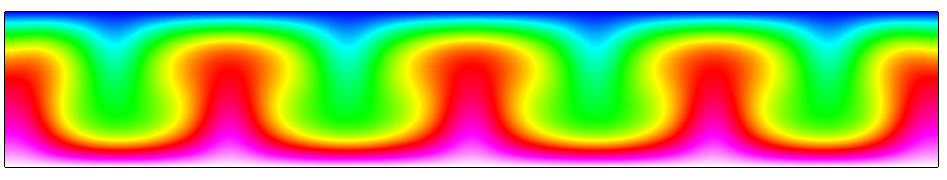
\includegraphics[width=0.8\textwidth]{temp}
\caption{zzz Temperature distribution at 260 s.}\label{fg:temp}
\end{figure} 

\subsection*{zzz Extra task:}

zzz If you have time you may try to solve the case with different parameters.

\hfill
